\documentclass[paperwidth=100cm,paperheight=160cm,portrait,fontscale=0.2941]{baposter}
\usepackage{lipsum} 
%841mm x 1189mm
\usepackage[font=small,labelfont=bf,hypcap=false]{caption} % Required for specifying captions to tables and figures
%\usepackage{cite}
\usepackage{booktabs} % Horizontal rules in tables
\usepackage{relsize} % Used for making text smaller in some places
%\usepackage[urlcolor  = blue]{hyperref}
%\graphicspath{{figures/}} % Directory in which figures are stored
\usepackage{multicol}
%\usepackage[style=ieee]{biblatex}
%\addbibresource{bib.bib}
\usepackage[utf8]{inputenc} 
%\usepackage{hyperref}
\usepackage{placeins}
\usepackage{epstopdf}
\usepackage{subcaption}
\usepackage[]{graphicx}
\usepackage{natbib}
\usepackage{times}

\bibliographystyle{abbrvnat}

\selectcolormodel{RGB} %<-- Add colour model defintion
\definecolor{bordercol}{RGB}{255,255,255}%{33,26,82} % Border color of content boxes
\definecolor{headercol1}{RGB}{255,255,255}%{33,26,82} % Background color for the header in the content boxes (left side)
%\definecolor{headercol2}{RGB}{5,2,82} % Background color for the header in the content boxes (right side)
\definecolor{headerfontcol}{RGB}{0,0,0}%{255,255,255} % Text color for the header text in the content boxes
\definecolor{boxcolor}{RGB}{255,255,255} % Background color for the content in the content boxes

\begin{document}
\graphicspath{{Pictures/}}
\background{ % Set the background to an image (background.pdf)

}

\begin{poster}{
grid=false,
headerheight=0.11\textheight,
borderColor=bordercol, % Border color of content boxes
headerColorOne=headercol1, % Background color for the header in the content boxes (left side)
%headerColorTwo=headercol2, % Background color for the header in the content boxes (right side)
headerFontColor=headerfontcol, % Text color for the header text in the content boxes
boxColorOne=boxcolor, % Background color for the content in the content boxes
headershape=rectangle, % Specify the rounded corner in the content box headers
headershade=plain,
headerfont=\Large\sf\bf, % Font modifiers for the text in the content box headers
textborder=rectangle,
background=user,
headerborder=open, % Change to closed for a line under the content box headers
boxshade=plain,
eyecatcher=true
}
%
%----------------------------------------------------------------------------------------
%	TITLE AND AUTHOR NAME
%----------------------------------------------------------------------------------------
%
%\vspace{2em}
% Eye Catcher Images to go left of your title.
{
\includegraphics[height=0.06\textheight]{aau_logo_new.eps}
} %will not show if put eyecatcher=false
% Title
{\vspace{2pt}
Estimating Auditory Filter Bandwidth using \\
Distortion Product Otoacoustic Emissions}
% Author
{
\vspace{3pt}
\normalsize{\textbf{Andreas H. Rukjær*, Sigurd van Hauen*, Rodrigo Pizarro Ordoñez** \& Dorte Hammershøi**}\\
**M.Sc. Students in Acoustics and Audio Technology, Aalborg University.\\ ***Signal and Information Processing, Department of Electronic Systems, Aalborg University.}

}
{

\includegraphics[height=0.06\textheight]{bearLOGO.eps}
}

%----------------------------------------------------------------------------------------
%	INTRODUCTION
%----------------------------------------------------------------------------------------
\headerbox{Introduction}
{name=introduction,column=0,row=0, span=1}
{\parskip 5pt   
    The present work is inspired by the findings of Christensen et al. (2015, 2017), which at low frequencies demonstrate the relation between the optimal $2f_1-f_2$ DPOAE stimulus ratio ($f_2/f_1$) and the Equivalent Rectangular Bandwidth (ERB), as defined by Glasberg and Moore (1990):
    \begin{equation}\label{eq:model}
        f_1 - f_2 = \gamma ERB(f_2),
    \end{equation}
The constant $\gamma$ was found experimentally to equal approximately 1.5 in Christensen et al. (2015, 2017) in normal hearing populations.  

}


\headerbox{Hypothesis}
{name=hypo,span=1,column=0,below=introduction, span=1}
{\parskip 5pt 
The auditory filter bandwidth  and the optimal DPOAE primary frequencies ratio depend on

1) the properties of the underlying morphology, and

2) the state of health in the underlying morphology.

If the optimal DPOAE primary frequencies ratio is equally affected by deterioration in the hearing as the auditory filter, DPOAE measurements may offer a fast alternative to the psychoacoustic test of auditory filter bandwidth. If not, it may hold individual information of the underlying morphology, and may serve as a calibration or normalization factor for the psychoacoustic (and other) individual measurements.


\textit{The purpose of the present investigation} was to further examine the individual relation between the psychoacoustic measure (ERB) and objective measure (optimal DPOAE stimulus ratio) at normal audiometric frequencies.
}

\headerbox{Methods}
{name=method,span=1,column=0,below=hypo, span=1}
{\parskip 5pt 
Auditory filter bandwidths and optimal DPOAE ratios were determined for 10~young (18-25~years), normal hearing (HL < 20~dB, MEP < $\pm$ 100~daPa) subjects around selected standard audiometric frequencies (1, 2, and 4~kHz).}


\headerbox{DPOAE measurements}
{name=OAE,span=1,column=0,below=method}
{\parskip 5pt 
An Etyomotic Research ER-10C probe system with a Roland UA-25EX sound card controlled through a customized MATLAB program were used to obtain the DPOAE measurements. The fixed-$f_2$ paradigm was utilized and stimulus levels were set at 65/45~dB~SPL. 


The DPOAE level at each of the eight selected $f_2$/$f_1$ primary ratios was computed as the mean energy of five separate measurements that were taken within one dip-to-dip bandwidth of the expected fine structure, according to Reuter and Hammershøi (2006).

~

    \begin{flushright}
    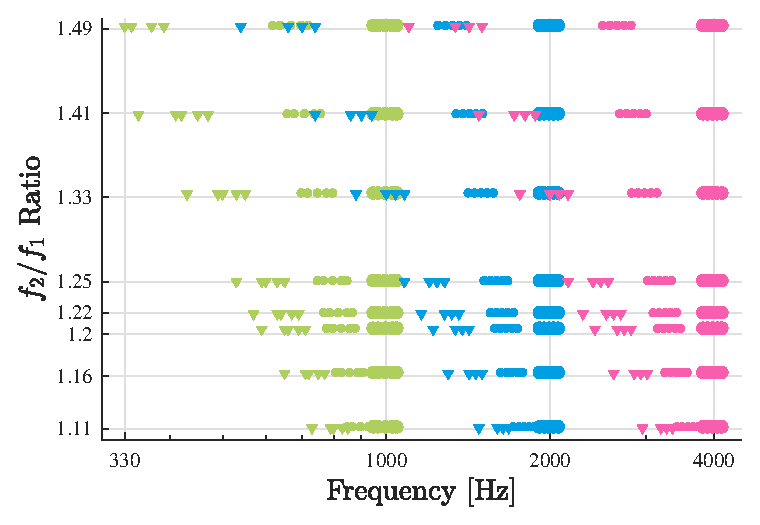
\includegraphics[width=0.95\linewidth]{RatioShow.eps}
    \end{flushright}
\vspace{-10pt}

    \textbf{Figure~1.} DPOAE frequencies included, $f_2$ (large circle), $f_1$ (small circle), 2$f_1$-$f_2$ (triangle).

}

\headerbox{Auditory Filter Determination}
{name=AF,span=1,column=0,below=OAE}
{\parskip 5pt

The noise and stimuli paradigm used in the auditory filter measurements, was a notched noise, with relative notch widths $\Delta f/f_c$ of 0, 0.05, 0.1, 0.2, 0.3 and 0.4. The noise masker was presented simultaneously with the stimulus tone with a 100~ms Hanning ramp applied to both start and end of the combined signal. Each noise and stimulus interval was presented with 0.5~s duration and a 0.25~s pause between intervals. The masker was presented at a level of 40 dB/Hz.

The psychoacoustic method used was an adaptive 2-alternative forced choice experiment. An initial step size of 8~dB was used, reducing it to half at each reversal, and stopping when the step size had converged to 2~dB. The threshold was calculated as the average of 6~reversals, after the step size had converged to 2~dB. A 2-down 1-up presentation strategy was used, so thresholds converge to approximately 70.7\% correct on the psychometric function. Subjects were given approximately 10~minutes under supervision for familiarization with the procedure.

%Thresholds were calculated using the final 6~reversals after the step size had converged to 2~dB, with the step size decreasing by 50~\% every reversal, starting at 8~dB. A 2-down 1-up method was used to ensure a higher convergence point on the psychometric function. Subjects were given approximately 10~minutes under supervision for familiarization with the procedure. 

The filter shapes were derived from the notched-noise experiment data using the PolyFit method from Patterson RD~(1976). A 3\textsuperscript{rd} order polynomial was fitted to the data.
}

\headerbox{DPOAE Results}
{name=DPOAEResults,span=1,column=1,aligned=introduction}
{\parskip 5pt
 

~

\begin{flushright}
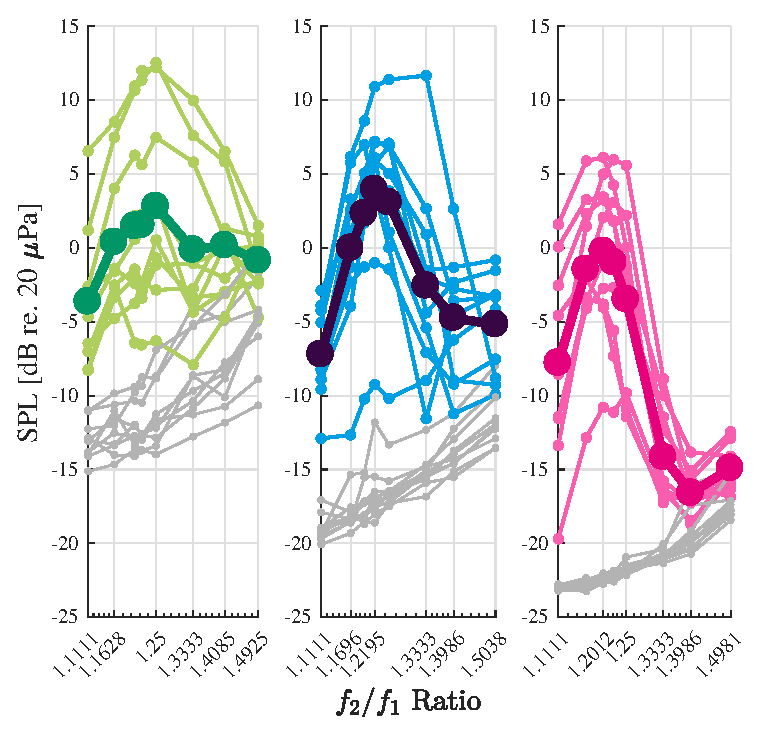
\includegraphics[width=0.95\linewidth]{pos_all_OAE.eps}
\end{flushright}
\vspace{-10pt}       

\textbf{Figure~2. }DPOAE levels as a function of primary frequency ratios. Thick lines represent group averages, and thin lines individual data. Grey lines represent the noise floor.

%~

The individual DPOAE levels display a bell-shaped dependency of stimulus ratio (Figure 2), allowing a fairly robust identification of individual optimal ratios (the maxima). The contours appear to be minimally affected by fine structures, suggesting that the method of averaging within a typical fine structure ripple bandwidth provides a simple alternative to advanced source separation algorithms.

} 

\headerbox{Optimal DPOAE ratio vs ERB, model}
{name=ERBmodel,span=1,column=1,below=DPOAEResults}
{\parskip 5pt
%Figure~3 shows group data for optimal DPOAE primary ratios plotted as a function of frequency together with the model relating DPOAE primary ratios to equivalent rectangular bandwidths (Eq.~\ref{eq:model}).

~

\begin{flushright}
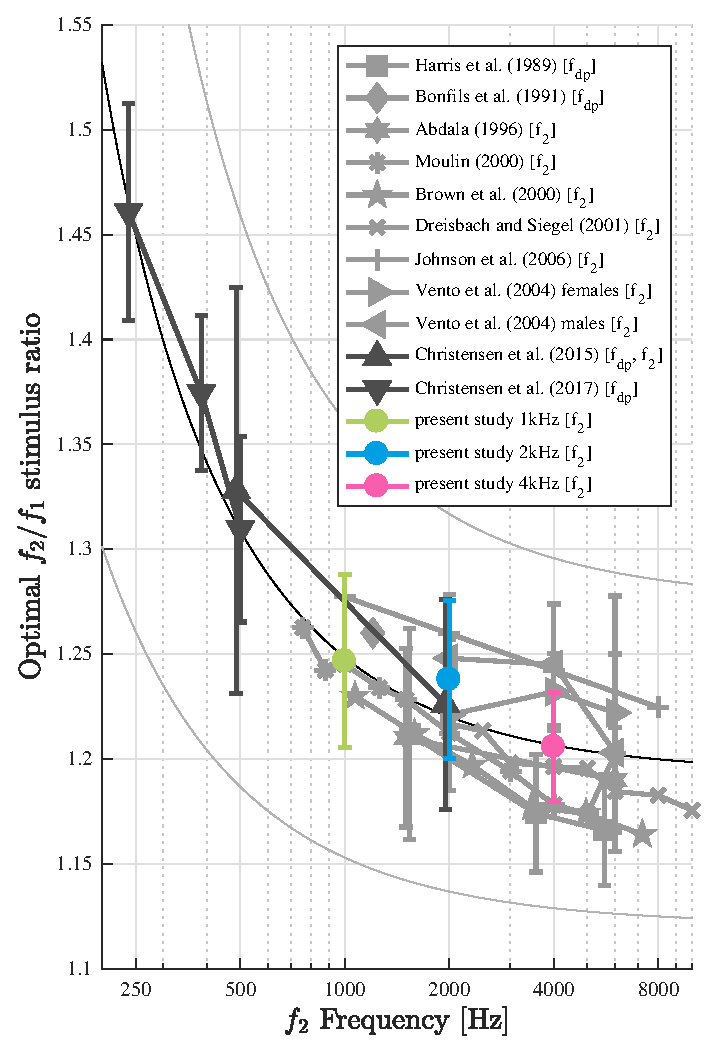
\includegraphics[width=0.95\textwidth]{LiteraturDataComp.eps}
\end{flushright}
\vspace{-15pt}
\textbf{Figure~3.} Optimal stimulus ratio (group mean $\pm$ one standard deviation) from present study (colors) fit a $\gamma$ value of 1.5 (underlying black line). Eq.~\ref{eq:model} with $\gamma = 1$ and $2$ are shown as the lower and upper grey lines. The square parentheses in the legend indicates whether the given study used a fixed-$f_2$ or fixed-$f_{dp}$ paradigm.

%~

Figure~3 shows that the group data from the present study (and from literature) comply well with an estimated $\gamma = 1.5$ in Eq.~\ref{eq:model}. 


}


\headerbox{Auditory Filter Results}
{name=AuditoryFResults,span=1,column=2,aligned=introduction}
{\parskip 5pt


~
\begin{flushright}
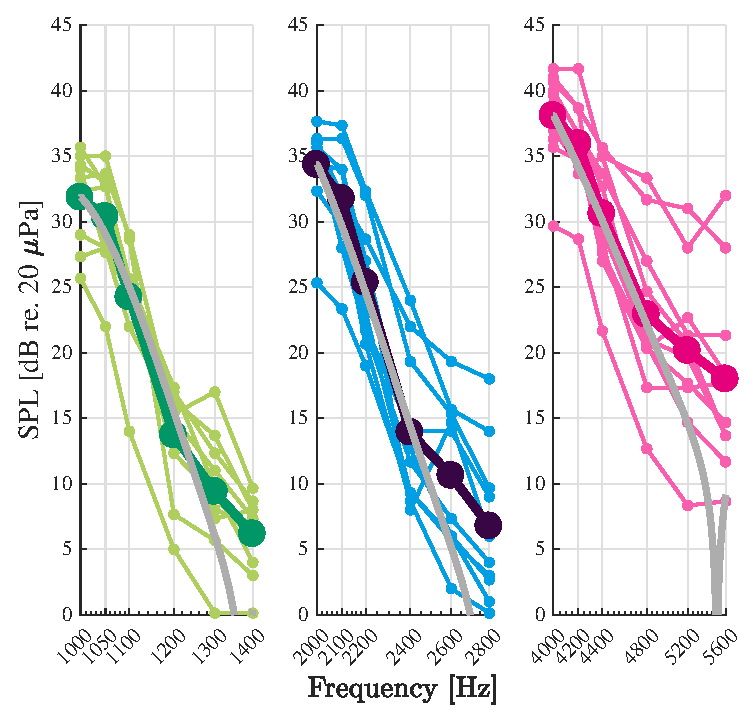
\includegraphics[width=0.95\linewidth]{pos_all_AF.eps}
\end{flushright}
\vspace{-2.7pt}

\textbf{Figure~4.} Level of tone at threshold as a function of masker bandwidth (level equal to 40~dB/Hz). Grey lines represent the estimated auditory filter shape derived from the mean data using the PolyFit method.

%~

Figure~4 shows that the wider the masking notch, the lower the masking effect on the stimulus tone. Figure~4 also shows that the slopes--with a few exceptions--are pretty steep, as would be expected for normal-hearing individuals.

}


\headerbox{Optimal ratio vs ERB, individual data}
{name=ERBdata,span=1,column=2,below=AuditoryFResults}
{\parskip 5pt
%Individual data for optimal DPOAE ratio and the individual equivalent rectangular bandwidhts.

~

\begin{flushright}
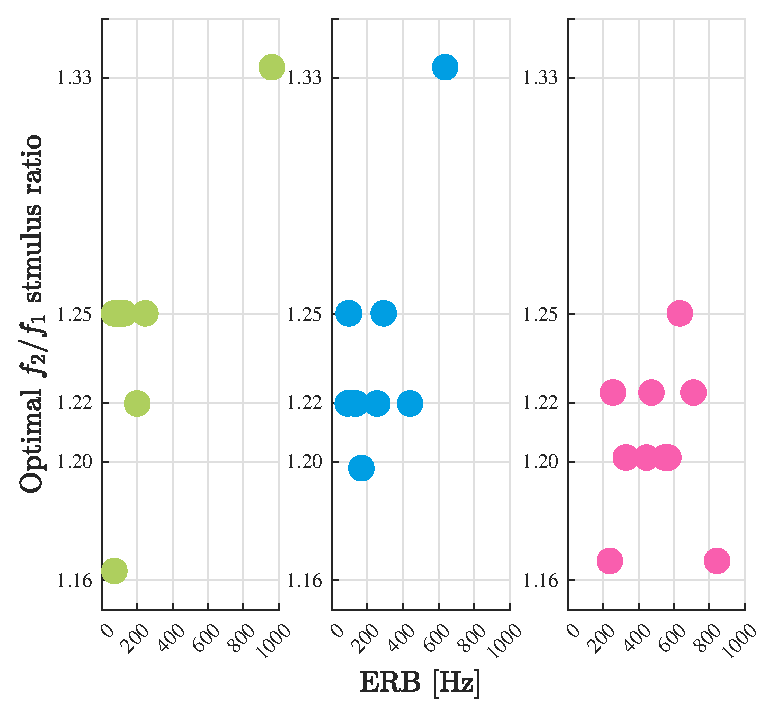
\includegraphics[width=0.95\textwidth]{ScatterBEAR.eps}
\end{flushright}
\vspace{-15pt}
\textbf{Figure~5.} Optimal DPOAE stimulus ratios versus the estimated equivalent rectangular bandwidths (estimated as the area under individually fitted polynomials of the measured data in Figure 4).

%~

Figure~5 shows that there may be a relation between optimal DPOAE stimulus ratio and auditory filter bandwidths, there is--however--too few points for generalization.

}


\headerbox{Conclusion}
{name=Conclusion,span=1,column=2,below=ERBdata}
{\parskip 5pt
Robust individual optimal DPOAE stimulus ratios were obtained through energy average of DPOAE measurements around three audiological frequencies. %The bandwidth chosen for this average corresponds to the expected ripple width of typical fine structures observed in high resolution measurements (Reuter et al., 2006).  

The present data confirms the optimal ratio relation to auditory filter bandwidth on group basis, and the relation can also be recognized for individual data. The data suggests that subjects with a broad auditory filter (high ERB estimate) also have the highest optimal ratio (Fig.~5, 1~and 2~kHz). In the same manner most subjects with low ERB estimates showed low optimal ratio, with one clear exception at 4~kHz (highest ERB estimate also gives a low optimal ratio).



}

\headerbox{Acknowledgements}
{name=akn,span=1,column=1,below=ERBmodel}
{\parskip 5pt
The support from the BEAR project and its partners, incl. funding from Innovation Fund Denmark is sincerely acknowledged, as is the grant from Danish Sound (the Research Talent Award 2017), and the support from the ISAAR organization. We also appreciate the collaboration by Raúl H. Sánchez López and the Hearing Systems Group from DTU for supplying MATLAB code and material for the notched-noise experiment.
}


\headerbox{References}
{name=references,column=2,below=Conclusion}
{
\renewcommand{\section}[2]{}%
%\parskip 5pt
 %   \bibliography{bib.bib}
%\tiny
\footnotesize
Abdala C (1996) JASA \textbf{100}(6):3726-3740.

Bonfils P et al. (1991) \textit{Arch Otolaryngol Head Neck Surg} \textbf{117}(10):1167–1171.

Brown DK et al. (2000) \textit{Hearing Res}. \textbf{145}(1-2):17-24.

Christensen AT et al. (2015) \textit{JASA} \textbf{137}(2):679-689.

Christensen AT et al. (2017) \textit{JARO} \textbf{18}(2):197-208.

Dreisbach LE and Siegel JH (2001) \textit{JASA} \textbf{110}(5):2456-2469.

Glasberg BR and Moore BC (1990) \textit{JASA} \textbf{47}:103-138.

Harris F et al. (1989) \textit{JASA} \textbf{85}(1):220–229

Johnson TA et al. (2006) \textit{JASA} \textbf{119}(1):418-428.

Moulin A (2000) \textit{JASA} \textbf{107}(3):1460–1470.

Patterson RD (1976) \textit{JASA} \textbf{59}(3):640-654.

Reuter K and Hammershøi (2006) \textit{JASA} \textbf{120}(1):270-279.

Vento BA et al. (2005) \textit{JASA} \textbf{115}(5):2138-2147.

}


%-------------------------------------------------------------------------

\end{poster}
\end{document}